\section{Metric Topologies}

  \begin{theorem}[Metric Topologies on Finite Sets]
    If $(X, d)$ is a finite metric space, then the metric topology on it is the discrete topology. 
  \end{theorem}
  \begin{proof}
    Take all pairwise points. 
  \end{proof}

  \begin{example}[Non-Metrizable Finite Spaces]
    Let $X = \{a, b c\}$. Then the topology 
    \begin{equation}
      \mathscr{T} = \{\emptyset, \{b\}, \{a, b\}, \{b, c\}, X \}
    \end{equation} 
    is not metrizable from the theorem above. 
  \end{example}


  Given a set $X$, we want a notion of a distance between two elements of $X$. This can be done with topologies, either by counting the number of open sets that contain $x, y \in X$ or by using notions of separability. We can also define it using a metric. 

  \begin{definition}
  The \textbf{metric} function $d: X \times X \longrightarrow \mathbb{R}$ is a structure endowed on a set $X$ with properties 
  \begin{enumerate}
      \item $\forall x, y \in X, \; d(x, y) \geq 0, \; \; d(x, y) = 0 \iff x = y$
      \item $d(x, y) = d(y, x)$ 
      \item $d(x, y) + d(y, z) \geq d(x, z)$
  \end{enumerate}
  Any function $d$ satisfying these three properties can be defined to be a metric. 
  \end{definition}

  Given a metric space $(X, d)$, consider the \textbf{$\epsilon$-ball centered at $x$}. That is, 
  \[B_d (x, \epsilon) \equiv \{y \in X \; | \; d(x, y) < \epsilon\}\]
  With $\epsilon$-balls, it is possible to construct an induced topology. However, note that a topology does not in general induce a metric. 

  \begin{definition}
  If $d$ is a metric on set $X$, then the collection of all $\epsilon$-balls $B_d (x, \epsilon)$ for $x \in X$ and $\epsilon > 0$ is a basis for a topology on $X$, called the \textbf{metric topology} induced by $d$. 
  \end{definition}

  While we will not prove this here, this set generated by $\epsilon$-balls does indeed satisfy the properties of a topology. We can rephrase the definition as follows 

  \begin{definition}
  A set $U$ is open in the metric topology induced by $d$ if and only if for each $y \in U$, there exists a $\delta > 0$ such that 
  \[B_d (x, \delta) \subset U\]
  \end{definition}
  Therefore, since there always exists a basis element that is a neighborhood of all points $x \in U$ completely within $U$, $U$ is by definition open. 

  \begin{example}
  The $L2$ metric induces the usual open ball topology in $\mathbb{R}^n$. In fact, this open ball topology implies the existence of the metric. 
  \end{example}

  \begin{example}
  Given a set $X$, induce the metric $d$ defined
  \[d(x, y) \equiv \begin{cases}
        1 & \text{if } x \neq y \\
        0 & \text{if } x = y
  \end{cases}\]
  This metric induces the discrete topology on $X$, since the basis elements of the open balls
  \[B_r (x) \equiv \{ y \in X \; | \; d(x, y) <r\}\]
  consists of two types of open sets. When $r \leq 1$, then $B_r (x) = x$ (since the radius is $0$). If $r > 1$, then the open set is the entire space $X$. 
  \end{example}

  In $\mathbb{R}$, note that every open ball is really just an interval. In fact, every open ball $(x - r, x + r)$ can be expressed with just two elements $a, b \in \mathbb{R}$, as $(a, b)$. Notice that this method of expressing an open set does not even require any metric! 

  Extending this to $\mathbb{R}^n$ would indicate that the topologies of $\mathbb{R}^n$ defined by the endpoint of the open intervals would not necessarily induce any metric either. Notice that these induced topologies is \textbf{not} the open ball topology, which must have an associated metric to it. Rather, this induced, non-metric topology is the box topology! While the box topology and the open ball topology are really the same topology, they are generated by inherently different bases. 

  \begin{definition}
  If $(X, \mathscr{T})$ is a topological space, $(X, \mathscr{T})$ is said to be \textbf{metrizable} if there exists a metric $d$ on $X$ that induces the topology $\mathscr{T}$ of $X$. That is, the set of all open balls of form
  \[B_r (x) \equiv \{ y \in X \; | \; d(x, y) < r \}\]
  is the basis of $\mathscr{T}$. A \textbf{metric space} is a metrizable space $X$ together with a specific metric $d$ that gives the topology of $X$. 
  \end{definition}

  Note that it makes no sense to say that a regular space $X$ is metrizable. A topology $\mathscr{T}$ must be given in addition to $X$ to determine whether $(X, \mathscr{T})$ is metrizable. Metrizability is always highly desirable attribute for spaces, and there are many existence theorems that proves metrizability given certain conditions. 

  \begin{definition}
  Let $(X, d)$ be a metric space with subset $A$. $A$ is \textbf{bounded} if there exists some number $M$ such that
  \[d (x, y) \leq M \text{ for all } x,y \in A\]
  If $A$ is bounded, the \textbf{diameter} of $A$ is defined to be the number
  \[\text{diam}\, A \equiv \sup{\{d(x, y) \; | \; x, y \in A\}}\]
  \end{definition}

  Note that boundedness on a set is not a topological property since it depends on the particular metric $d$ that is used for $X$. For example, we can construct the following metric that makes every subset in $X$ bounded. 

  \begin{definition}
  Let $(X, d)$ be a metric space. We define a second metric $\Tilde{d}$ on $X$ such that
  \[\Tilde{d} (x, y) \equiv \min{\{d(x, y), 1\}}\]
  $\Tilde{d}$ is called the \textbf{standard bounded metric corresponding to $d$}. 
  \end{definition}

  If we construct open balls with this metric, it is easy to see that they consist of all open balls with radius less than or equal to 1. That is, the topology $\mathscr{T}$ consists of all open balls
  \[\mathscr{T} \equiv \{B_r (x) \; | \; x \in X, r \leq 1\}\]
  It is also clear that the topology induced by $\Tilde{d}$ is the same as the topology induced by $d$! The significance of this construction of the standard bounded metric is that we can now work with a basis consisting of bounded elements, which is much nicer than a basis of open balls that can have arbitrarily large radii.  

  \begin{lemma}
  Let $d$ and $d^\prime$ be two metrics on the set $X$, with $\mathscr{T}$ and $\mathscr{T}^\prime$ the topologies that they induce, respectively. Then $\mathscr{T}^\prime$ is finer than $\mathscr{T}$ if and only if for each $x \in X$ and each $\epsilon > 0$, there exists a $\delta > 0$ such that
  \[B_{d^\prime} (x, \delta) \subset B_d (x, \epsilon)\]
  That is, for every open ball at $x$ with respect to metric $d$, there exists a smaller open ball at $x$ with respect to metric $d^\prime$. 
  \end{lemma}

  \begin{corollary}
  Given two topologies $\mathscr{T}$ and $\mathscr{T}^\prime$ of a set $X$, if $\mathscr{T}$ is finer than $\mathscr{T}^\prime$ and $\mathscr{T}^\prime$ is finer than $\mathscr{T}$, then $\mathscr{T} = \mathscr{T}^\prime$. That is, two topologies that have the same level of "fineness" are the same topologies. 
  \end{corollary}

  \begin{definition}
  Similar to the Euclidean, or L-2 metric of $\mathbb{R}^n$, we define the \textbf{Euclidean/L-2} norm on $\mathbb{R}^n$ as
  \[||x||: \bigg( \sum_{i=1}^n x_i \bigg)^{\frac{1}{2})}\]
  \end{definition}

  \begin{definition}
  The \textbf{L-$\infty$ metric}, also know as the \textbf{square metric}, on $\mathbb{R}^n$ is defined 
  \[\rho(x, y) \equiv \max{\{|x_1 - y_1|, ..., |x_n - y_n|\}}\]
  \end{definition}

  We now introduce a metrization theorem on $\mathbb{R}^n$. 

  \begin{theorem}
  The topologies on $\mathbb{R}^n$ induced by the Euclidean metric $d$ and the square metric $\rho$ are the same as the product topology on $\mathbb{R}^n$. 
  \end{theorem}
  \begin{proof}
  Given $x, y \in \mathbb{R}^n$, simple algebra shows that 
  \begin{align*}
      & \rho(x, y) \leq d(x, y) \leq \sqrt{n} \rho(x, y) \\
      & \;\;\;\; \implies \forall x, \epsilon, \; B_d (x, \epsilon) \subset B_\rho (x, \epsilon) \text{ and } B_\rho (x, \frac{\epsilon}{\sqrt{n}}) \subset B_d (x, \epsilon)
  \end{align*}
  But
  \[\{ B_\rho (x, \epsilon) \; | \; x \in \mathbb{R}^n, \epsilon \in \mathbb{R}\} = B_\rho (x, \frac{\epsilon}{\sqrt{n}}) \; | \; x \in \mathbb{R}^n, \epsilon \in \mathbb{R}\}\]
  which means that the metric topology induced by $d$ is the same as the metric topology induced by $\rho \implies$ the two topologies are the same. We know that the topology induced by $\rho$ is the same as the product topology since 
  \[\prod_{i=1}^n (x_i - r, x_i + r) = \bigcup_{k=1}^n \mathbb{R}^{k-1} \times (x_k - r, x_k + r) \times \mathbb{R}^{n-k}\]
  \end{proof}
  With this theorem, we have proved that given a topological space $\mathbb{R}^n$ with the product topology, there exists a metric (the Euclidean and square metric) that induces this product topology. 

  Visually, we can see that every open ball in $(\mathbb{R}^n, d)$ (with the Euclidean metric) is the form to the left, while an open ball in $(\mathbb{R}^n, \rho)$ (with the square metric) is of form on the right. 
  \begin{center}
  \begin{tikzpicture}[scale=0.5]
      \draw [dashed] (1,0) circle [radius=2];
      \draw [dashed] (6,-2) rectangle (10,2);
      \draw [fill] (1,0) circle [radius=0.05];
      \node [above left] at (1,0) {x};
      \draw (1,0)--(3,0);
      \node [above] at (1.5,0) {r};
      \draw [fill] (8,0) circle [radius=0.05];
      \node [below right] at (8,0) {x};
      \draw (8,0)--(10,0);
      \draw (8,0)--(8,2);
      \node [right] at (8,1) {r};
      \node [above] at (9,0) {r};
  \end{tikzpicture}
  \end{center}
  Clearly, we can form any open set of any "shape" using any arbitrary combination of these "circles" or "squares," indicating that they generate the same topology. 

  We can attempt to extrapolate these formulas to $\mathbb{R}^\omega$ by defining
  \begin{align*}
      & d(x, y) \equiv \bigg(\sum_{i=1}^\infty (x_i - y_i)^2 \bigg)^{\frac{1}{2}} \\
      & \rho(x, y) \equiv \sup{\{|x_i - y_i|\}}
  \end{align*}
  However, the metrics do not in general map to elements of $\mathbb{R}$, since the sequence $(x_i - y_i)_{i \in \mathbb{N}}$ could diverge. Therefore, we can redefine the metric $\rho$ to the following bounded one. 
  \[\Tilde{\rho} (x, y) \equiv \sup{\{\Tilde{d}(x_i, y_i)\}}\]
  where $\Tilde{d}$ is the standard bounded metric on $\mathbb{R}$. Clearly,
  \[0 \leq \Tilde{\rho}(x, y) \leq 1\]
  $\Tilde{\rho}$ is indeed a metric on $\mathbb{R}^\omega$, but unfortunately, it does not induce the product topology. We extend this definition to arbitrary $\mathbb{R}^J$. 

  \begin{definition}
  Given an indexed set $J$ with points $x, y \in \mathbb{R}^J$, we define
  \[\Tilde{\rho} \equiv \sup{\{\Tilde{d}(x_\alpha, y_\alpha)\;|\; \alpha \in J\}}\]
  with $\Tilde{d}$ the standard bounded metric on $\mathbb{R}$. $\Tilde{\rho}$ is called the \textbf{uniform metric on $\mathbb{R}^J$}, which induces the \textbf{uniform topology}. 
  \end{definition}

  The uniform topology on $\mathbb{R}^J$ is finer than the product topology, and they are different if $J$ is infinite. Clearly, $0 \leq \Tilde{p} (x, y) \leq 1$, meaning that given the open ball
  \[B_r (x) \equiv \{y \in \mathbb{R}^J \;|\; \Tilde{p}(y, x) < r\}\]
  if $r \geq 1$, then $B_r (x) = \mathbb{R}^J$ and if $r<1$, then $B_r (x)$ consists of the $n$-dimensional box with "radius" $r$, where $n = \dim{\mathbb{R}^J}$. In $\mathbb{R}^3$, each basis element is a cube centered at $x$ with side lengths $2r$.
  \begin{center}
  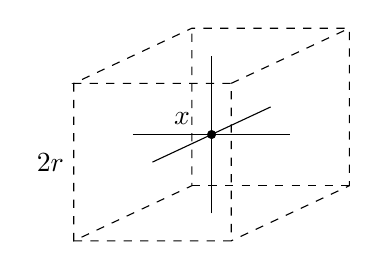
\begin{tikzpicture}
      \draw[dashed] (0,0)--(2,0)--(2,2)--(0,2)--(1.5,2.7)--(3.5,2.7)--(3.5,0.7)--(2,0);
      \draw[dashed] (2,2)--(3.5,2.7);
      \draw[dashed] (0,2)--(0,0)--(1.5,0.7)--(1.5,2.7);
      \draw[dashed] (1.5,0.7)--(3.5,0.7);
      \draw (1,1)--(2.5,1.7);
      \draw (0.75,1.35)--(2.75,1.35);
      \draw (1.75,0.35)--(1.75,2.35);
      \draw[fill] (1.75,1.35) circle (0.05);
      \node[above left] at (1.6,1.35) {$x$};
      \node[left] at (0,1) {$2r$};
  \end{tikzpicture}
  \end{center}

  The next theorem gives us a metric that induces the product topology on infinite dimensional $\mathbb{R}^\omega$ by slightly modifying the uniform metric on $\mathbb{R}$. However, with the box topology $\mathbb{R}^\omega$ is not metrizable. 

  \begin{theorem}
  Let $\Tilde{d} (a, b) \equiv \min{\{|a-b|, 1\}}$ be the standard bounded metric on $\mathbb{R}$. If $x, y \in \mathbb{R}^\omega$, we define
  \[ D(x, y) \equiv \sup{\Big\{ \frac{\Tilde{d}(x_i, y_i)}{i}\Big\}}\]
  Then, $D$ is a metric that induces the product topology on $\mathbb{R}^\omega$. 
  \end{theorem}
  It is easy to see that $0 \leq D(x, y) \leq 1$. So, given the open ball
  \[B_r (x) \equiv \{y \in \mathbb{R}^\omega \; | \; D(x, y) < r\}\]
  $B_r (x) = \mathbb{R}^\omega$ if $r > 1$. When $r \leq 1$, 
  \[B_r (x) \equiv (y-r, y+r) \times (y-2r, y+2r) \times ... = \prod_{k=1}^\infty (y - k r , y + k r)\]
  Visually, we take a cross section of this box and look at the slice within $\mathbb{R}_1 \times \mathbb{R}_2$, where the subscripts represent the first and second terms of $x$. 
  \begin{center}
  \begin{tikzpicture}
      \node[below left] at (0,0) {$y$};
      \draw[fill] (0,0) circle (0.05);
      \draw[<->] (0, -2)--(0,2);
      \draw[<->] (-3,0)--(3,0);
      \draw[fill] (-2,0) circle (0.05); 
      \draw[fill] (2,0) circle (0.05); 
      \draw[fill] (0,1) circle (0.05); 
      \draw[fill] (0,-1) circle (0.05); 
      \node[above left] at (-2,0) {$-2$};
      \node[above right] at (2,0) {$2$};
      \node[above right] at (0,1) {$1$};
      \node[below right] at (0,-1) {$-1$};
      \draw[fill] (0, 0.7) circle (0.05);
      \draw[fill] (1.4, 0) circle (0.05);
      \node[above left] at (0,0.7) {$r$};
      \node[below right] at (1.4,0) {$2r$};
      \draw[dashed] (-1.4, -0.7) rectangle (1.4,0.7);
      \node[right] at (0,2) {$\mathbb{R}_1$};
      \node[above] at (3,0) {$\mathbb{R}_2$};
  \end{tikzpicture}
  \end{center}

  \begin{proposition}
  Every metric topology satisfies the Hausdorff Axiom.
  \end{proposition}
  \begin{proof}
  If $x$ and $y$ are distinct points of $(X, d)$, then letting
  \[\varepsilon = \frac{1}{2} d(x, y)\]
  the triangle inequality implies that $B_\varepsilon (x)$ and $B_\varepsilon (y)$ are disjoint. 
  \end{proof}

  We now define continuity with the metric using the $\epsilon - \delta$ definition and connect it to the topological definition of continuity. Given 2 metric spaces $(X, d)$ and $(Y, \rho)$ with $f: X \longrightarrow Y$, it is clear that $x, y \in X \implies f(x), f(y) \in Y$. Given that $d(x, y) < \delta$ for a certain $\delta$, we can guarantee that $\rho(f(x), f(y)) < \epsilon$ for some $\epsilon$. In fact, we can make $\epsilon$ as small as we wish, and there will always be a $\delta > 0$ that satisfies $d(x, y) < \delta \implies \rho(f(x), f(y)) < \epsilon$.  

  \begin{definition}
  A function $f: (X, d) \longrightarrow (Y, \rho)$ between metric spaces is continuous at $p$ if for all $\epsilon > 0$, there exists a $\delta > 0$ such that 
  \[ d(x, p) < \delta \implies \rho ( f(x), f(p)) < \epsilon\]
  If $f$ is continuous at all $p \in X$, then we can say that $f$ is continuous.
  \end{definition}

  \begin{theorem}
  Now, we endow $(X, d), (Y, \rho)$ their open ball topologies, leading to the sets $(X, \tau_X, d)$ and $(Y, \tau_Y, \rho)$, respectively. Given function $f: X \longrightarrow Y$, we claim that $f$ is continuous according to the $\epsilon - \delta$ definition if and only if $f^{-1}(U) \in \tau_{X}$ for any $U \in \tau_Y$. That is, these two definitions of continuity are equivalent. 
  \end{theorem}

  \begin{proof}
  ($\rightarrow$) Assume $f$ is continuous according to the $\epsilon - \delta$ definition. Let $U$ be any open set in $Y$ containing the point $y$, and let $x$ be an element in $f^{-1}(U)$ such that $y = f(x)$. We must prove that $f^{-1}(U)$ is also open. Since open sets contain neighborhoods (e.g. open balls) of all of its points, we can claim that, since $U$ is open by assumption, there exists an open ball $B_y$ around $y$ with radius $\epsilon > 0$. This guarantees the existence of a point $z \in U$ such that $\rho(y, z) < \epsilon$ for any $\epsilon > 0$ that we choose. Since $f$ is continuous, for every $\epsilon >0$ that we chose previously, there exists a $\delta >0$ such that $d(x, w) \implies \rho(f(x), f(w)) < \epsilon$. Since $\rho(f(x), f(w)) < \epsilon$, we can conclude that $f(w) \in B_y \subset U$ when $d(x, w) < \delta$. Therefore, $d(x, w) < \delta \implies w \in f^{-1}(U)$. But this is equivalent to saying that if $w \in B_(x, \delta)$, then $w \in f^{-1}(U)$, which means that every single point $x \in f^{-1}(U)$ contains an open ball neighborhood fully contained in $f^{-1}(U)$. So, by definition, $f^{-1}(U)$ is open. 


  ($\leftarrow$) Assume $f^{-1}(U)$ is open when $U$ is an open set in $Y$, i.e. $f$ is continuous under the topological definition. Let us define the open ball 
  \[ B(f(x), \epsilon) \equiv \{ y \in Y \; | \; \rho(f(x), y) < \epsilon\} \in \tau_Y\]
  By our assumption, $f^{-1} \big( B(f(x), \epsilon) \big)$ is an open set in $\tau_X$, and clearly, $x \in f^{-1} \big( B(f(x), \epsilon) \big)$ since $f^{-1}$ maps the point $f(x) \in B(f(x), \epsilon)$ to $x \in f^{-1} \big( B(f(x), \epsilon) \big)$. But since $f^{-1} \big( B(f(x), \epsilon) \big)$ is open, we can construct an open ball around $x$ with radius $\delta$ fully contained within the open set. Moreover, by selecting a point $p \in B(f(x), \delta) \subset f^{-1}\big( B(f(x), \epsilon) \big)$, we can guarantee that $f(p) \in B(f(x), \epsilon)$. This is precisely the $\epsilon - \delta$ definition of continuity. That is, given an $\epsilon > 0$ to be the radius of an open ball $B(f(x), \epsilon)$ in $Y$, we can always choose a $\delta > 0$ to be the radius of the open ball $B(x, \delta)$ in $X$ that is fully contained within the preimage of $B(f(x), \epsilon)$. In mathematical notation, 
  \[ p \in B(x, \delta) \subset f^{-1} \big( B(f(x), \epsilon) \big) \implies f(p) \in f\big( B(x, \delta) \big) \subset B(f(x), \epsilon)\]
  or equivalently in terms of metrics,
  \[ d(x, p) < \delta \implies \rho (f(x), f(p)) < \epsilon\]
  \end{proof} 

  \begin{definition}
  A sequence $(x_\alpha)$ of points in topological space $(X, \mathscr{T})$ is said to \textbf{converge} to the point $x \in X$ if for every neighborhood $U$ of $x$ there exists a $N \in \mathbb{N}$ such that
  \[x_n \in U \text{ for all } n \geq N\]
  Furthermore, if a sequence converges, it converges to one point provided that $X$ is Hausdorff! For if $(x_\alpha)$ converges to $x$ and if $y \neq x$, then we need only choose disjoint neighborhoods of $y$ and $x$ to prove that $(x_\alpha)$, by definition, is not convergent to $y$.
  \end{definition}

  Visually, we can think of each $x_N$ in the sequence as a point in a metric space $(X, d)$. To see if $\{ x_i \}$ converges to a point $l \in X$, we construct an open ball $B(l, \epsilon)$ and see if all points $x_i$ after a certain $i = m$ lie within $B (l, \epsilon)$. If this can be done for all $\epsilon > 0$, then $\{ x_i \}$ converges to $l$, or 
  \[\lim_{i \to \infty} \{ x_i \} = l \]

  \begin{example}
  The space $(0,1)$ with the nested interval topology is not Hausdorff. In fact, it is impossible to distinguish 2 points $x, y$ if $x, y \in (0, \frac{1}{2})$, meaning that the sequence
  \[\frac{1}{10}, \frac{2}{10}, \frac{1}{10}, ...\]
  converges to both $\frac{1}{10}$ and $\frac{2}{10}$.
  \end{example} 

  We can extend the applications of the Bolzano Weierstrass Lemma from analysis to metric spaces in general with the following lemma. 

  \begin{lemma}[Sequence Lemma]
  If $X$ be a topological space with $A \subset X$. If there exists a sequence of points of $A$ that converges to $x$, then $x \in \bar{A}$. The converse is true if $X$ is metrizable. 
  \end{lemma}
  \begin{proof}
  $(\rightarrow)$ Our hypothesis says that $x$ is a limit point of $A$, which by definition means that $x \in \bar{A}$. \\
  $(\leftarrow)$ Assuming $X$ is metrizable and $x \in \bar{A}$, let $d$ be a metric for the topology of $X$. Then, for every $n \in \mathbb{N}$, let us define a sequence of open neighborhoods of $x$ to be
  \[\big(B_{\frac{1}{n}} (x) \big)\]
  Since $x \in \bar{A}$, there exists a point 
  \[x_n \in A \cap B_{\frac{1}{n}} (x) \text{ for all } n \in \mathbb{N}\]
  This sequence $(x_n)$ that we have proved must exist converges to $x$. 
  \end{proof}

  \begin{theorem}
  Let $f: X \longrightarrow Y$ and let $X$ be metrizable. $f$ is continuous if and only if for every convergent sequence $(x_n) \rightarrow x$ of $X$, the following sequence of $Y$ converges to $f(x)$. That is, 
  \[\big( f(x_n) \big) \longrightarrow f(x)\]
  \end{theorem}

  We introduce additional methods of constructing continuous functions. 

  \begin{lemma}
  The addition, subtraction, and multiplication operations are continuous functions from $\mathbb{R} \times \mathbb{R} \longrightarrow \mathbb{R}$, and the quotient operation is a continuous function from $\mathbb{R} \times (\mathbb{R} \setminus \{0\}) \longrightarrow \mathbb{R}$. 
  \end{lemma}
  \begin{proof}
  Standard $\epsilon-\delta$ proof. 
  \end{proof}

  \begin{theorem}
  If $X$ is a topological space, and if $f, g: X \longrightarrow \mathbb{R}$ are continuous, then $f + g$, $f-g$, and $f \cdot g$ are also continuous. $f / g$ is continuous if $g(x) \neq 0$ for all $x \in X$. 
  \end{theorem}

  \begin{definition}
  Let $f_n: X \longrightarrow Y$ be a sequence of functions from the set $X$ to the metric space $(Y, d)$. The sequence $(f_n)$ is said to \textbf{converge uniformly} to the function $f: X \longrightarrow Y$ if, given $\epsilon > 0$, there exists a $N \in \mathbb{N}$ such that
  \[d\big( f_n(x), f(x)\big) < \epsilon\]
  for all $n \geq N$ and for all $x \in X$. 
  \end{definition}

  \begin{theorem}[Uniform Limit Theorem]
  Let $f_n: X \longrightarrow Y$ be a sequence of continuous functions from topological space $X$ to a metric space $Y$. If $f_n$ converges uniformly to $f$, then $f$ is continuous. 
  \end{theorem}
  \begin{proof}
  $(\rightarrow)$ Trivial. \\
  $(\leftarrow)$ Let $V$ be open in $Y$, and let $x_0$ be a point in $f^{-1} (V)$. It suffices to prove that for every $x_0 \in f^{-1} (V)$, there exists a neighborhood $U$ of $x_0$ such that $U \subset F^{-1} (V)$ or equivalently, $F(U) \subset V$. 

  Let $y_0 = f(x_0)$. Since $Y$ is a metric space with metric $d$, we know that there exists an $\epsilon$-ball $B_\epsilon (y_0)$ such that
  \[B_\epsilon (y_0) \subset V\]
  Then, using uniform convergence, we can choose $N \in \mathbb{N}$ such that for all $n \geq N$ and all $x \in X$, 
  \[d \big( f_n (x), f(x) \big) < \frac{\epsilon}{4}\]
  which also applies at the point $x = x_0$. 
  \[d \big( f_n (x_0), f(x_0) \big) < \frac{\epsilon}{4}\]
  Using continuity of $f_n$, choose a neighborhood $U$ of $x_0$ such that $f_n$ carries $U$ into the open $\epsilon/2$-ball centered at $f_n (x_0)$ (note that $f_n (x_0) \neq y_0$), meaning that if $x \in U$
  \[d \big( f_n (x), f_n (x_0) \big) < \frac{\epsilon}{2}\]
  Adding the three inequalities and using the triangle inequality, we get the fact that if $x \in U$, then 
  \[d \big( f(x), f(x_0) \big) < \epsilon\]
  meaning that the $f(U) \subset B_\epsilon (x_0) \subset V$. 
  \end{proof}

  Visually, the three inequalities represent the following open balls in $V \subset Y$.
  \begin{center}
  \begin{tikzpicture}[scale=0.6]
      \draw[dashed, teal] (0,0) circle [radius=8];
      \draw[fill] (0,0) circle [radius=0.05];
      \draw[fill] (-1.5,0.5) circle [radius=0.05];
      \draw[dashed, purple] (0,0) circle [radius=2];
      \draw[dashed, purple] (-1.5,0.5) circle [radius=2];
      \node[right] at (0.3,0) {$f(x_0)$};
      \node[above right] at (-1.5,0.5) {$f_N (x_0)$};
      \draw[dashed, blue] (-1.5,0.5) circle [radius=4];
      \draw[fill] (-4,3) circle [radius=0.05];
      \draw[dashed, purple] (-4,3) circle [radius=2];
      \node[right] at (-4,3) {$f_N (x)$};
      \draw[fill] (-5.5, 3.7) circle [radius=0.05];
      \node[above left] at (-5,4.5) {$f(x)$};
      \draw[-, thick] (-5.5, 3.7)--(-4,3)--(-1.5,0.5)--(0,0);
      \draw[->, thick, purple] (0,0)--(0,-2);
      \draw[->, thick, blue] (-1.5,0.5)--(-1.5,-3.5);
      \node[right, purple] at (0,-1) {$\epsilon / 4$};
      \node[left,blue] at (-1.5,-1.5) {$\epsilon / 2$};
      \draw[->, thick, teal] (0,0)--(6.128, 5.1416);
      \node[below right, teal] at (3.064, 2.57) {$\epsilon$};
  \end{tikzpicture}
  \end{center}

  \begin{proposition}
  In a metric space $(X, d)$, a set is \textbf{closed} if the limit of every convergent subsequence in $X$ lies in $X$. That is, $X$ contains all of its limit points. 
  \end{proposition}

